\documentclass[11pt,a4paper]{article}

\usepackage[utf8]{inputenc}
\usepackage[T1]{fontenc}
\usepackage{lmodern}
\usepackage[margin=2.5cm]{geometry}
\usepackage{amsmath,amssymb}
\usepackage{booktabs}
\usepackage{graphicx}
\usepackage{xcolor}
\usepackage{listings}
\usepackage[numbers,sort&compress]{natbib}
\usepackage[colorlinks=true,linkcolor=blue!50!black,citecolor=blue!50!black,urlcolor=blue!50!black]{hyperref}
\usepackage{caption}
\usepackage{enumitem}
\usepackage{microtype}
\emergencystretch=2em

\graphicspath{{../figures/}}
\setlist{nosep,leftmargin=*}
\lstset{basicstyle=\ttfamily\footnotesize,columns=fullflexible,frame=single,framerule=0.3pt,breaklines=true}
\newcommand{\code}[1]{\texttt{#1}}

\title{\textbf{Clustbench: A Reproducible, Trajectory-Instrumented,\\ Self-Extending Benchmark for Clustering Algorithms}}
\author{Ashail Maharaj\\\small\url{https://github.com/Ashail33/clustbench}}
\date{October 2026}

\begin{document}
\maketitle

\begin{abstract}
Clustering algorithms are hard to compare. Published evaluations differ in
datasets, sample sizes, metrics, hyperparameters and hardware, and few report
runtime or memory in a reproducible way. We present \emph{Clustbench}, an
open-source benchmark harness that makes the comparison mechanical. A YAML
configuration expands into a Cartesian grid of tasks over synthetic,
real-world, time-series, graph and adversarial datasets with known ground
truth. Every registered algorithm, whether native Python or any executable
speaking a four-field JSON protocol, runs on the same data, and each run is
recorded as one schema-validated row holding external validity (ARI, NMI),
internal validity (silhouette, Davies--Bouldin, Dunn) and resource use (wall
time, memory delta, CPU and I/O). Results are aggregated by average ranks and
a Friedman test. Clustbench adds three things that existing clustering
benchmarks do not provide together. First, a \emph{trajectory layer} logs every
step of an iterative algorithm as a $(\text{state}, \text{action},
\text{cost}, \Delta\text{cost})$ record, so the optimisation process becomes
data. Second, machine-readable \emph{algorithm cards} give theoretical cost
and quality predictions next to the measured values. Third, the benchmark's own
output is the training set for a \emph{self-extending} layer of learned
algorithm selectors that retrain automatically when new algorithms or datasets
are added. On the current release (47 algorithms, 19 dataset families,
72 tasks, 3{,}354 result rows) the Friedman test rejects equal performance
decisively ($\chi^2 = 1189$, $p \approx 7\times10^{-219}$). No single
algorithm wins every dataset family. A separate out-of-distribution benchmark
shows that the selectors that rank highest in-distribution lose
0.11--0.13 ARI on unseen regimes, which is the main methodological lesson the
harness surfaced.
\end{abstract}

\section{Introduction}

Clustering has no single correct objective~\cite{kleinberg2002impossibility},
so the practical question \emph{which algorithm should I use on this data?}
is answered empirically. The empirical literature is fragmented. Each paper
picks its own datasets, scale, hyperparameter budget, metrics and hardware,
and wall time and memory are usually reported anecdotally if at all. A
white paper on benchmarking in cluster analysis~\cite{vanmechelen2018benchmarking}
names these problems and calls for neutral, reproducible comparisons.

The author's MEng research assignment~\cite{maharaj2024review} reviewed big-data
clustering methods, proposed a four-way taxonomy (sampling/partitioning,
ensemble, parallel/distributed and incremental methods), and benchmarked one
representative of each category: S$^5$C~\cite{matsushima2019s5c},
PWCC~\cite{alguliyev2020weighted}, MapReduce-style parallel
$k$-means~\cite{zhao2009parallel} and mini-batch $k$-means~\cite{sculley2010web}.
Its closing recommendation was a \emph{centralised database for clustering
research} that would let practitioners find the right model for their data and
infrastructure. That study's experiments were limited by compute: the full
factorial grid exceeded the available notebook quota. Clustbench turns the
recommendation into software and keeps the grid cheap to re-run.

\paragraph{Contributions.}
\begin{enumerate}
  \item \textbf{A language-agnostic harness} (\S\ref{sec:design}) that expands
  a declarative configuration into a task grid, runs any number of algorithms
  on identical data, and writes one tidy, schema-validated record per run
  together with resource measurements, average ranks and a Friedman test.
  \item \textbf{A trajectory layer} (\S\ref{sec:trajectory}) that records the
  step-by-step optimisation of iterative algorithms as state--action--reward
  tuples. To our knowledge this is the first clustering benchmark to treat the
  \emph{search process} as a first-class output.
  \item \textbf{Algorithm cards, a gap finder and a mutator}
  (\S\ref{sec:cards}) that encode each algorithm's mechanism, inductive biases
  and complexity in machine-readable form, predict cost and quality from them,
  and search the fingerprint space for regimes no registered algorithm covers.
  \item \textbf{A benchmark suite} (\S\ref{sec:suite}) of more than thirty
  dataset generators across convex, non-convex, heterogeneous-density,
  outlier-heavy, low-rank high-dimensional, real tabular, time-series, graph
  and deliberately adversarial regimes, and a registry of 50 algorithm
  implementations.
  \item \textbf{An empirical study} (\S\ref{sec:results}) that includes
  in-distribution, held-out-seed and out-of-distribution evaluations. It
  documents a failure mode of learned algorithm selection that only the
  out-of-distribution split exposes.
\end{enumerate}
A companion paper~\cite{clustbenchalgos} describes the new algorithms
developed with the harness. This paper covers the harness, the suite and what
the benchmark measures.

\section{Related work}

\paragraph{Clustering benchmarks.} Van Mechelen et
al.~\cite{vanmechelen2018benchmarking} set out principles for neutral
benchmarking in cluster analysis. Gagolewski~\cite{gagolewski2022framework}
proposed a framework and curated battery of low-dimensional benchmark datasets
with reference partitions, distributed as a Python package that is \emph{also}
named \code{clustbench}. The two projects are independent and complementary:
Gagolewski's work is a dataset battery with reference labels, while ours is a
run harness with resource measurement, trajectory capture and learned
selection. Gagolewski's batteries could be loaded through our dataset
interface. Fahad et al.~\cite{fahad2014survey} gave an empirical taxonomy of
big-data clustering algorithms that the author's review built
on~\cite{maharaj2024review}.

\paragraph{Synthetic data with ground truth.} MDCGen~\cite{iglesias2019mdcgen}
generates multidimensional clustering datasets with controllable outliers,
noise and density. Clustbench reimplements an MDCGen-style generator and adds
shape generators (moons, circles, spirals, Swiss roll, rings), heavy-tailed and
imbalanced mixtures, and adversarial families.

\paragraph{Statistical comparison.} We follow Dem\v{s}ar's
recommendation~\cite{demsar2006statistical} of average ranks with the
Friedman test~\cite{friedman1937use} for comparing many algorithms over many
datasets.

\paragraph{Algorithm selection and meta-learning.} Choosing an algorithm from
dataset features is Rice's algorithm selection
problem~\cite{rice1976algorithm}. It has been studied as meta-learning in
general~\cite{brazdil2009metalearning,pfahringer2000landmarking} and for
clustering
specifically~\cite{desouto2008ranking,ferrari2015clustering}, and is used as
warm-starting in AutoML~\cite{feurer2015efficient}. Clustbench's learned
routers are instances of this idea. The contribution here is the
infrastructure that makes them self-extending: the router training set
\emph{is} the benchmark output, so it grows whenever the benchmark runs.

\section{Design}\label{sec:design}

\subsection{Task grid}
A benchmark is a YAML file. Each dataset entry lists value sets for sample
size $n$, dimension $d$, target cluster count $k$, compactness and
generator-specific knobs (outlier count, noise points, density, outlier
extremity). The harness takes the Cartesian product of every list and crosses
it with a list of seeds:
\begin{lstlisting}
datasets:
  - id: mdcgen
    n_samples: [500]
    n_features: [10]
    k_targets: [3, 5]
    outliers: [0, 100]
algorithms:
  - {name: kmeans,  kind: python,   entry: kmeans,  params: {n_init: 3}}
  - {name: mine,    kind: external, entry: ./bin/run_my_algo}
seeds: [1, 2, 3]
\end{lstlisting}
A task is uniquely identified by
$(\text{dataset}, n, d, k, \text{compactness}, \text{outliers}, \text{noise},
\text{density}, \text{seed})$. Every algorithm sees the identical array for a
given task.

\subsection{Algorithm interface}
Native algorithms subclass a small abstract base class, register themselves
under a string key, and implement \code{fit\_predict(X, k)}, which returns
an \code{AlgoResult} with integer labels, an optional dictionary of
algorithm-specific extras, and an optional trajectory. External algorithms in
any language are supported through a JSON-over-stdin protocol. The harness
writes the task to a \code{.npy} file and sends
\begin{lstlisting}
{"data_path": "...", "k": 5, "params": {...},
 "artifacts_dir": "...", "labels_path": "..."}
\end{lstlisting}
on standard input. The executable writes integer labels to
\code{labels\_path} and may print a JSON object of extras to standard output.
That is the entire protocol.

\subsection{Records and resource measurement}
Each (algorithm, task) pair produces one record validated by a Pydantic schema
(Appendix~\ref{app:schema}). Resource use is measured with \code{psutil}
around the \code{fit\_predict} call: wall-clock time, resident-set-size
delta, user and system CPU time, and read/write bytes where the platform
exposes them. Metrics are computed by one function shared by all algorithms:
ARI~\cite{hubert1985comparing} and NMI~\cite{strehl2002cluster} against
ground truth; silhouette~\cite{rousseeuw1987silhouettes} (sub-sampled above
5{,}000 points), Davies--Bouldin~\cite{davies1979cluster} and
Dunn~\cite{dunn1973fuzzy} as internal indices; plus compactness and
separation. The results table is flat (one column per metric), so a
leaderboard is a one-line query in pandas or DuckDB. A crashing algorithm is
logged and skipped and does not abort the sweep. In the 4{,}332-row
comprehensive run, 156 (3.6\%) runs failed this way and every other result was
kept.

\subsection{Aggregation}
For each metric, algorithms are ranked within every task (rank 1 = best,
ties averaged). Ranks are averaged across tasks, and the Friedman
statistic is computed over the tasks on which every algorithm produced a
result~\cite{demsar2006statistical}. The summary is written to
\code{summary.json} and also recomputed in the browser by the dashboard, so
adding an algorithm never requires changing analysis code.

\subsection{The trajectory layer}\label{sec:trajectory}
Iterative clustering algorithms are sequential decision processes. At each
step they observe a state (centroids, medoids, an assignment, a mixture's
parameters), take an action (reassign, move a centroid, swap a medoid, merge
two clusters), and observe a change in objective. Clustbench lets an algorithm
return a list of \code{Step} objects that are persisted as a Parquet
trajectory table with one row per step:
\[
  (\textit{run\_id}, \textit{task}, t, \; s_t, \; a_t, \; c_t, \; \Delta c_t = c_t - c_{t-1}, \; \textit{accepted}_t).
\]
Here $s_t$ is a numeric state snapshot, $a_t$ is a typed action (e.g.\
\code{\{"type": "swap", "out": 17, "in": 42\}}), $c_t$ is the scalar
objective, and the boolean records whether a proposed action was accepted
(local-search methods such as CLARANS~\cite{ng2002clarans} reject most
proposals). The negative of $\Delta c_t$ is a natural reward. Concatenated
across runs, trajectories are a dataset for value models over
$(s, a) \mapsto \Delta c$, for learned proposal distributions, and for
imitation learning of clustering policies. The companion
paper~\cite{clustbenchalgos} trains such a policy. In the current release, 36
of the 47 benchmarked algorithms emit trajectories, and the in-distribution
run stores 2{,}569 of them. Figure~\ref{fig:traj} shows three.

\begin{figure}[t]
  \centering
  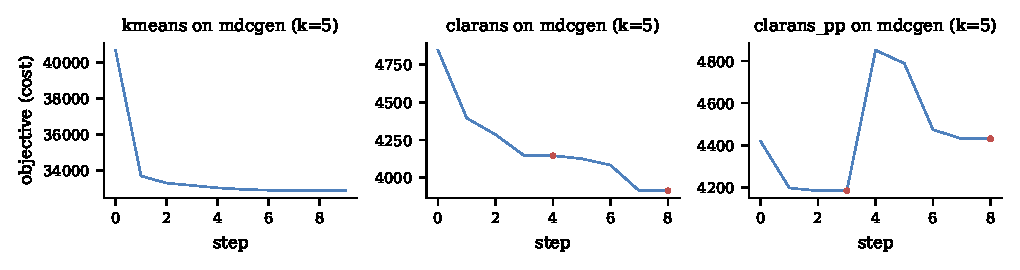
\includegraphics[width=\linewidth]{trajectories.pdf}
  \caption{Trajectory records for one MDCGen task ($n{=}500$, $d{=}10$,
  $k{=}5$, 100 injected outliers, seed 1). $k$-means descends monotonically in
  a few EM steps; CLARANS and its $k$-means++-seeded variant take many local
  swap steps, and red dots mark rejected proposals.}
  \label{fig:traj}
\end{figure}

\subsection{Algorithm cards, gap finder and mutator}\label{sec:cards}
Each registered algorithm has an \emph{algorithm card}: its taxonomy family,
a set of mechanism tags (e.g.\ \code{kpp\_init}, \code{graph\_laplacian},
\code{posterior\_weighting}), a set of inductive biases (e.g.\
\code{convex\_clusters}, \code{non\_convex\_capable}, \code{needs\_k}),
callables for time and memory complexity in $(n, d, k)$, a hyperparameter
space, and whether $k$ is an input. Cards serve three purposes.
\begin{itemize}
  \item \textbf{Theoretical predictions.} Every result row carries three
  predicted columns (\code{theoretical\_*}: wall time, memory and an ARI
  upper bound) next to the measured values. After
  calibration, predicted wall time landed within $0.6$--$1.5\times$ of measured
  for every algorithm. The deviations are diagnostic: mean shift's ratio of
  $0.59$ shows that its card's $O(n^2)$ is pessimistic for the bin-seeded
  implementation.
  \item \textbf{Gap finding.} Given dataset fingerprints (effective
  dimension, convexity, outlier fraction, density skew and similar), the gap
  finder scores every card's predicted ARI upper bound and reports regimes
  where the best card falls below a threshold. Those regimes become new
  datasets.
  \item \textbf{Mutation.} The mutator applies four operators
  (\code{swap\_mechanism}, \code{add\_bias}, \code{crossover},
  \code{stack}) to cards and keeps candidates whose predicted mean ARI beats
  the best existing card by at least 0.02. The top candidate in a 200-step
  random search was implemented and benchmarked~\cite{clustbenchalgos}.
\end{itemize}
The card predictions are an \emph{ordering} heuristic, not a calibrated
estimate. The mutator predicted $0.926$ ARI for its proposed hybrid, which
actually reached $0.747$ (\S\ref{sec:discussion}).

\subsection{Dashboard and continuous evaluation}
A static, dependency-free HTML dashboard served from the repository's
\code{docs/} folder reads the results and trajectory JSON. It shows
per-algorithm comparisons, a filterable per-task leaderboard, rank and
Friedman tests computed in the browser, and a trajectory viewer. A build
script converts any run directory into dashboard JSON, so refreshing the
public leaderboard is one command plus a commit.

\section{The benchmark suite}\label{sec:suite}

\paragraph{Datasets.} Generators share one contract,
$\text{DataSpec} \mapsto (X, y)$, with $y = -1$ for injected outliers and
noise. They fall into six groups.
\begin{itemize}
  \item \emph{Convex and near-convex synthetic:} isotropic blobs, an
  MDCGen-style mixture~\cite{iglesias2019mdcgen} with outlier, noise and
  density knobs, sheared (anisotropic) blobs, imbalanced blobs, hierarchical
  nested Gaussians, and heavy-tailed Student-$t$ mixtures.
  \item \emph{Non-convex synthetic:} moons, concentric circles, spirals, Swiss
  roll, S-curve, rings and mixed shapes.
  \item \emph{Heterogeneous density and contamination:} varying density and
  \code{extreme\_outliers}, which uses a tunable outlier extremity.
  \item \emph{Low rank in high dimension:} an inverse-PCA generator that places
  cluster means in a low-dimensional latent space and projects them to
  50--200 ambient dimensions.
  \item \emph{Real tabular data:} Iris~\cite{fisher1936use}, Wine, Breast
  Cancer, Digits (projected to 16 dimensions), Olivetti faces, Glass,
  Vehicle, Segment, Yeast and E.~coli~\cite{dua2019uci}.
  \item \emph{Other modalities:} time series (UCR
  ECG200 and Trace~\cite{dau2019ucr}, plus a synthetic set) reduced to a
  16-dimensional summary of 8 statistics, 4 FFT magnitudes and 4
  autocorrelations; graph nodes (Zachary's karate
  club~\cite{zachary1977information} and a stochastic block
  model~\cite{holland1983stochastic}) reduced to 6 centralities and 10
  Laplacian eigenvectors.
  \item \emph{Adversarial:} \code{PowerLawStudentT} (anisotropic Student-$t$
  components with Zipf-distributed masses, whose first two moments look
  Gaussian) and \code{VariableDensityBridges} (dense cores with Cauchy tails
  joined by thin Poisson bridges, so no single $\varepsilon$ works). Both were
  designed specifically to break the learned selectors.
\end{itemize}

\paragraph{Algorithms.} The registry holds 50 implementations. The classical
baselines are $k$-means with $k$-means++ seeding~\cite{lloyd1982least,arthur2007kmeanspp},
mini-batch $k$-means~\cite{sculley2010web}, MapReduce-style parallel
$k$-means~\cite{zhao2009parallel}, BIRCH~\cite{zhang1996birch}, Ward
agglomerative~\cite{ward1963hierarchical}, Gaussian mixtures via
EM~\cite{dempster1977maximum}, spectral clustering~\cite{ng2002spectral},
DBSCAN~\cite{ester1996density}, OPTICS~\cite{ankerst1999optics}, mean
shift~\cite{comaniciu2002mean}, CLARANS~\cite{ng2002clarans},
Chameleon~\cite{karypis1999chameleon}, an unweighted consensus vote,
PWCC~\cite{alguliyev2020weighted} and S$^5$C~\cite{matsushima2019s5c}. The
last four of the thesis's representatives (parallel $k$-means, mini-batch,
PWCC and S$^5$C) cover its four taxonomy categories. The remaining entries are
new algorithms described in the companion paper~\cite{clustbenchalgos}:
basis-mixture models, targeted fixes, synthesised pipelines, a graph-native
method, ten learned selectors and a behaviour-cloned agent.

\paragraph{Evaluation splits.}
\begin{itemize}
  \item \emph{In-distribution} (\code{benchmark.paper.demo.yaml}): 19
  dataset configurations, seeds $\{1,2,3\}$, $n \le 1000$; this is the split
  the learned selectors train on.
  \item \emph{Held-out seeds} (\code{benchmark.holdout.yaml}): the same
  shapes with seeds $\{11,12,13\}$, which removes seed-level memorisation.
  \item \emph{Out-of-distribution} (\code{benchmark.unseen.yaml}): seven
  configurations with $(n, d, k)$ tuples, outlier extremities and seeds
  ($100$--$102$) absent from training, e.g.\ MDCGen at $d{=}25, k{=}7$, moons
  embedded in $d{=}5$, inverse-PCA at $d{=}150$, and outlier extremity 10.
\end{itemize}

\section{Results}\label{sec:results}

All numbers below come from the data committed in the repository
(\code{docs/data} and \code{docs/data\_unseen}). The figures are regenerated
from those files by the script \code{make\_figures.py} in
\code{paper/scripts}.

\subsection{Overall leaderboard}
The in-distribution run covers 47 algorithms on 72 tasks (24 task variants
from 19 dataset configurations, $\times$ 3 seeds), giving 3{,}354 result
rows. Figure~\ref{fig:ranks} shows average ARI ranks. Over the 64 tasks
that every algorithm completed, the Friedman test gives $\chi^2 = 1188.8$
($p = 7.1\times10^{-219}$). The top seven positions are learned selectors
(\S\ref{sec:ood} qualifies this). The strongest single algorithms are the
graph-Laplacian methods: LMM (average rank 17.0, mean ARI 0.813) and spectral
clustering (17.6, 0.809).

\begin{figure}[t]
  \centering
  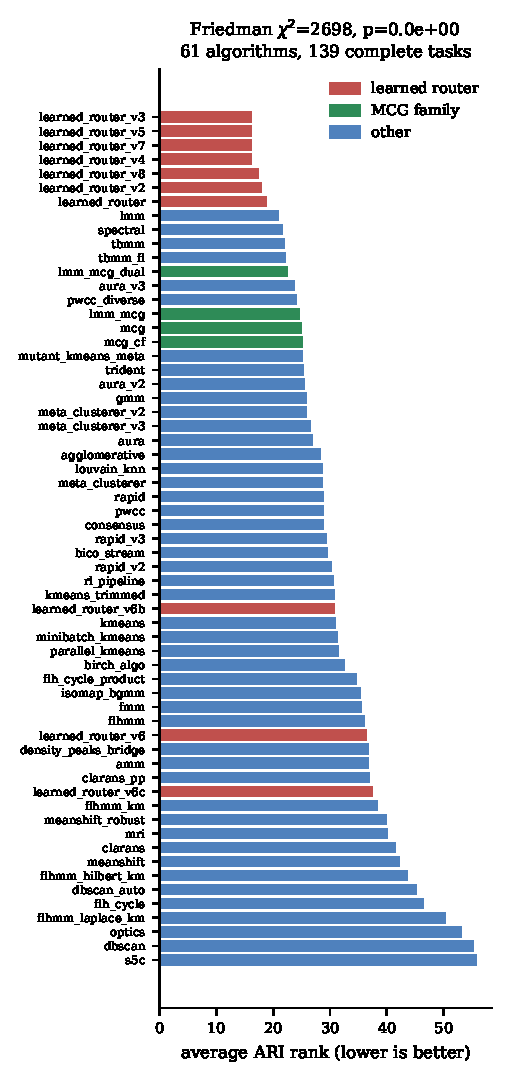
\includegraphics[width=0.55\linewidth]{rank_bars.pdf}
  \caption{Average ARI rank over the in-distribution split. Red bars are
  learned selectors, which are trained on this split (leave-one-out at the
  task level).}
  \label{fig:ranks}
\end{figure}

\subsection{No algorithm dominates}
Figure~\ref{fig:heatmap} breaks ARI down by dataset family for sixteen
representative algorithms. Four populations emerge.
\begin{itemize}
  \item \emph{Convex-only} methods ($k$-means family, BIRCH, Ward, PWCC with
  $k$-means-style bases) score $\approx 1$ on blobs and $\approx 0$ on
  circles.
  \item \emph{Graph-Laplacian} methods (spectral, LMM, AURA-v3) solve
  circles but reach only 0.52--0.61 on moons.
  \item \emph{Graph-community} clustering (\code{louvain\_knn}) is the only
  non-selector above 0.95 on moons, and scores 0.772 on the karate graph,
  where the next best non-selector reaches 0.506.
  \item \emph{Gaussian mixtures} are best on Iris (0.904) and Wine (0.559),
  and within 0.01 of the best on Breast Cancer (0.794).
\end{itemize}
Every family has a different winner, which is the regime-mismatch problem that
motivates algorithm selection.

\begin{figure}[t]
  \centering
  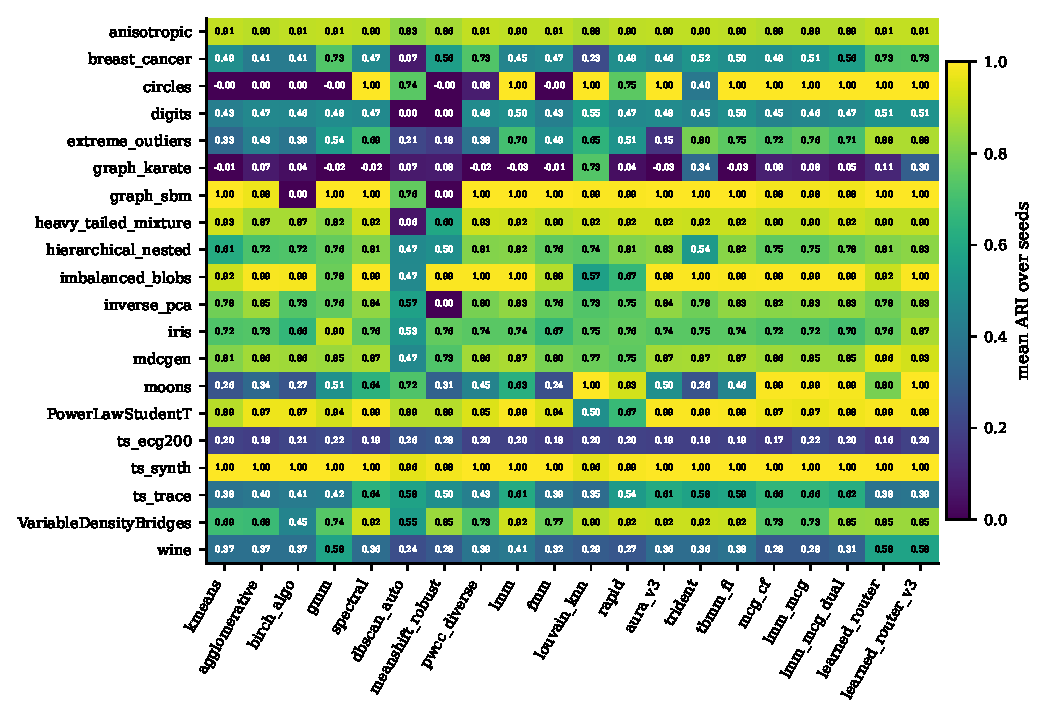
\includegraphics[width=\linewidth]{heatmap.pdf}
  \caption{Mean ARI over seeds for each dataset family (rows) and
  representative algorithm (columns), in-distribution split. The blank cell is
  a run that failed and was logged.}
  \label{fig:heatmap}
\end{figure}

\subsection{Failure modes are few and recurrent}
The algorithm analysis bundled with the repository diagnoses each algorithm
along four axes: scaling, clean-data quality, outlier robustness and shape
adaptability. Six failure modes account for almost every weakness: outlier
sensitivity of mean-based updates, non-convex shape failure of Voronoi-cell
methods, quadratic scaling, hyperparameter brittleness, local-minimum search,
and wrong data assumptions. Some examples:
\begin{itemize}
  \item With 100 outliers injected into 500 points, $k$-means loses 32\% of its
  ARI and mean shift loses 59\% (its bandwidth estimate is inflated by the
  outliers). GMM loses only 15\%, because its posterior-weighted mean update
  gives outliers little influence.
  \item DBSCAN with a fixed $\varepsilon{=}0.8$ in $d{=}10$ returns one cluster
  on every task (ARI 0.00).
  \item S$^5$C scores 0.27 on isotropic blobs because it assumes a union of
  linear subspaces, but gains $+0.36$ on sheared data where that assumption
  holds.
\end{itemize}
Measured log--log wall-time slopes between $n{=}200$ and $n{=}2000$ range
(excluding DBSCAN's degenerate one-cluster runs) from 0.33 (mini-batch
$k$-means) through 1.01 (BIRCH, the only high-quality method
that scales linearly in this range) to 1.78 (the MRI-inspired method).

Because the harness runs originals and variants side by side, it can test
whether a diagnosed fix helps. Table~\ref{tab:fixes} reports five one-line
fixes. Replacing DBSCAN's constant $\varepsilon$ with the $k$-distance knee
of Ester et al.~\cite{ester1996density} lifts mean ARI by 0.59. One fix barely
moved: trimming 10\% of points per $k$-means iteration cannot absorb a 20\%
outlier rate. Two fixes introduced new failures. $k$-means++ seeding of CLARANS
is biased \emph{toward} outliers, because seeding probability is proportional
to squared distance. The auto-$\varepsilon$ knee is itself contaminated by
outliers.

\begin{table}[t]
  \centering
  \caption{Diagnosed one-line fixes, mean ARI over the 16-task demonstration
  sweep (round 2 snapshot).}
  \label{tab:fixes}
  \begin{tabular}{llrrr}
    \toprule
    original & fixed variant & ARI before & ARI after & $\Delta$ \\
    \midrule
    \code{dbscan} & \code{dbscan\_auto} ($k$-distance knee) & 0.000 & 0.589 & $+0.589$ \\
    \code{meanshift} & \code{meanshift\_robust} (trimmed bandwidth) & 0.470 & 0.622 & $+0.151$ \\
    \code{clarans} & \code{clarans\_pp} ($k$-means++ seeding) & 0.581 & 0.656 & $+0.075$ \\
    \code{pwcc} & \code{pwcc\_diverse} (heterogeneous bases) & 0.702 & 0.751 & $+0.049$ \\
    \code{kmeans} & \code{kmeans\_trimmed} (10\% trim) & 0.701 & 0.703 & $+0.003$ \\
    \bottomrule
  \end{tabular}
\end{table}

\subsection{Generalisation: the split that changes the conclusion}\label{sec:ood}
The learned selectors are trained on the benchmark's own results. Their
in-distribution scores use task-level leave-one-out, which removes exact
self-matches but still lets a sibling seed of the same configuration serve
as a near neighbour. Clustbench therefore ships two stricter splits.

On the \emph{held-out-seed} split, every algorithm scored slightly
\emph{higher} than in-distribution (the new seeds were easier), and the
early selectors' gaps ($-0.015$, $-0.020$) matched those of non-learning
methods (LMM $-0.027$). No seed-level memorisation was detectable.

The \emph{out-of-distribution} split changes the picture
(Figure~\ref{fig:ood}). The four selectors that lead the in-distribution
board lose between 0.115 and 0.128 ARI: v3, v5 and v7 fall from about 0.91 to
0.753 and v4 to 0.734. The simplest selector (v1, a $k$-nearest-neighbour vote
over seven fingerprint features) \emph{improves} to 0.840. LMM, which has no
learned component, ranks first at 0.845, followed by v1, AURA-v2/v3 (0.837,
0.835) and \code{louvain\_knn} (0.825). The more capacity a selector has to fit
the training fingerprint distribution, the more it overfits it. The split that
reveals this costs one configuration file, and we argue such a split should be
a default part of any benchmark that also trains selectors on its own output.

\begin{figure}[t]
  \centering
  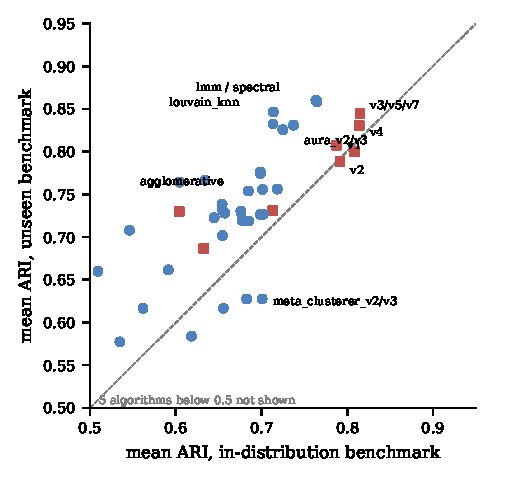
\includegraphics[width=0.5\linewidth]{ood_scatter.pdf}
  \caption{Mean ARI in-distribution vs.\ on the out-of-distribution split for
  the 42 algorithms run on both. Squares are learned selectors. Points below
  the diagonal lost accuracy off-distribution; the highest-ranked selectors
  lose the most.}
  \label{fig:ood}
\end{figure}

\subsection{The self-extending loop}
Clustbench's learned selectors read the committed results file when they are
imported, so adding an algorithm and re-running the benchmark retrains them
with no code change. This has happened twice.
\begin{itemize}
  \item A domain enlargement exposed the karate graph as a regime where every
  algorithm scored below 0.43 ARI. A graph-community algorithm,
  \code{louvain\_knn}, was added and scored 0.772 there. On the next run, every
  fingerprint-based selector dispatched to it on that task, and the mean ARI of
  the best selectors rose by 0.029--0.038. No selector code changed between the
  two runs.
  \item Adding three discovery-agent algorithms, five datasets and two more
  selectors raised the stacker selector's mean ARI from 0.871 to 0.912, again
  without selector code changes.
\end{itemize}
The intelligence accumulates in the data, not the code.

\section{Discussion}\label{sec:discussion}

\paragraph{What the harness made cheap.} Re-running every algorithm on every
task is a single command. The research loop therefore became: diagnose a
failure, ship a variant, re-rank against everything. The companion paper's
fifteen rounds of algorithm development each cost one configuration change
and one sweep. The latest round, in which LLM agents proposed, implemented,
integrated and benchmarked three algorithms and five datasets, took about 17
minutes of wall clock.

\paragraph{Learning beats predicting from biases.} Card-based predictions are
useful for ordering candidate mutations, but their magnitudes are not
calibrated. The mutator's top proposal was predicted at 0.926 ARI and measured
at 0.747. Card-predicted upper bounds also \emph{under}estimate how well
classical methods generalise: spectral clustering's actual unseen ARI of
0.775 exceeds its card bound of 0.614. Selectors trained on measured results
outperform selectors driven by inductive-bias arithmetic, but only within
their training distribution.

\paragraph{Threats to validity.}
\begin{itemize}
  \item \emph{Scale.} Most tasks have $n \le 1000$. Wall-time slopes are
  measured only up to $n{=}2000$, so the constant-cost phases of some methods
  make their slopes look sub-linear. Clustbench's design does not limit $n$,
  but the reported sweeps were sized for continuous integration.
  \item \emph{Seeds and statistics.} There are three seeds per configuration.
  The Friedman test is over-powered with 47 algorithms; post-hoc pairwise
  tests (e.g.\ Nemenyi) are needed before claiming that any two adjacent
  algorithms differ.
  \item \emph{Timing.} Wall time and RSS deltas come from a single shared
  machine and include Python overhead; they support order-of-magnitude
  comparisons, not micro-benchmarks.
  \item \emph{Selector leakage.} In-distribution selector scores are
  optimistic by construction; only the out-of-distribution split is an
  honest estimate.
  \item \emph{Data provenance.} The UCR loader falls back to a synthetic
  generator if every mirror is unreachable. The inverse-PCA generator depends
  on a companion package and was disabled in the latest in-distribution run.
  Rows record their \code{dataset\_source}.
  \item \emph{Coverage.} Round-14 and later algorithms, and GMM, were not
  re-run on the out-of-distribution split.
  \item \emph{Ground-truth outliers.} Injected outliers carry label $-1$ in
  the ground truth and are scored as their own class by ARI and NMI.
\end{itemize}

\section{Conclusion}
Clustbench turns ``which clustering algorithm should I use?'' into a
reproducible, re-runnable measurement. It records full resource usage and the
step-by-step optimisation trajectory, ships theoretical predictions next to
measurements, and feeds its own output to selectors that improve when the
registry grows. Its most useful result so far is a caution: selectors that
lead the leaderboard on the distribution they were trained on can trail a
classical graph-Laplacian mixture model on data they have not seen. Future work
is larger-$n$ sweeps, post-hoc pairwise testing, importing external dataset
batteries such as Gagolewski's~\cite{gagolewski2022framework}, and
using the trajectory corpus to train learned components inside algorithms
rather than selectors between them.

\paragraph{Availability.} Code, configurations, committed results, the live
dashboard (\url{https://ashail33.github.io/clustbench/}) and the scripts that
regenerate every figure in this paper are at
\url{https://github.com/Ashail33/clustbench}.

\bibliographystyle{unsrtnat}
\bibliography{../references}

\appendix
\section{Record schema}\label{app:schema}
\begin{table}[h]
  \centering\small
  \resizebox{\linewidth}{!}{%
  \begin{tabular}{ll}
    \toprule
    field & description \\
    \midrule
    \code{algo}, \code{dataset\_id} & algorithm and dataset keys \\
    \code{n\_samples}, \code{n\_features}, \code{k\_target} & task shape \\
    \code{compactness}, \code{outliers}, \code{noise}, \code{density}, \code{seed} & generator knobs \\
    \code{wall\_time\_s}, \code{rss\_delta\_mb} & wall-clock time, memory delta \\
    \code{cpu\_user\_s}, \code{cpu\_system\_s}, \code{read\_bytes}, \code{write\_bytes} & CPU and I/O \\
    \code{ari}, \code{nmi} & external validity \\
    \code{silhouette}, \code{davies\_bouldin}, \code{dunn}, \code{compactness}, \code{separation} & internal validity \\
    \code{n\_clusters\_found}, \code{extra} & output cardinality, algorithm extras \\
    \code{n\_steps}, \code{trajectory\_path} & trajectory length and Parquet path \\
    \code{theoretical\_*} & card-based predictions (wall time, RSS, ARI bound) \\
    \bottomrule
  \end{tabular}}
\end{table}
Trajectory rows add \code{run\_id}, \code{step\_idx}, \code{cost},
\code{delta\_cost}, \code{accepted}, \code{action} and \code{state}.

\end{document}
